%\documentclass[10pt,handout]{beamer}
\documentclass[10pt]{beamer}
\usepackage[ngerman]{babel}
\usepackage[utf8]{inputenc}
\usepackage{amsmath}
\usepackage{amssymb}
\usepackage{listings} 
\usepackage{mathtools}
\usepackage{ulem}
\usepackage{hyperref}
\usetheme{Boadilla}

\parskip 10pt

\lstset{language=Python, tabsize=4, basicstyle=\footnotesize, showstringspaces=false,mathescape=true} 
\lstset{literate=%
  {Ö}{{\"O}}1
  {Ä}{{\"A}}1
  {Ü}{{\"U}}1
  {ß}{{\ss}}1
  {ü}{{\"u}}1
  {ä}{{\"a}}1
  {ö}{{\"o}}1
} 
\begin{document}
\title{Algorithmus und Programm}   
\author{Informatik} 
\date{ } 

\frame{\titlepage} 

%-------------
\begin{frame}[fragile]
\textbf{Informatik} ist die Wissenschaft von der systematischen Verarbeitung von Informationen, insbesondere der automatischen Verarbeitung mit Hilfe von Rechenanlagen (Wikipedia).  

Wir beschäftigen uns zu Beginn mit Algorithmen und deren Programmierung in Python. 

Ein \textit{Algorithmus} ist eine endlich lange Vorschrift, bestehend aus Einzelanweisungen. \pause

Ein in einer Computersprache formulierter Algorithmus heißt \textit{Programm}.  

Eine umgangssprachliche Formulierung, die die Struktur des Algorithmus deutlich macht, nennen wir  \textit{Pseudocode}. 

\end{frame}

\begin{frame}[fragile]

Der Collatz-Algorithmus in Pseudocode
\begin{lstlisting} 
lies x ein    
setze z auf 0
solange x $\ne$ 1 tue
    wenn x gerade
          dann halbiere x
    sonst 
          verdreifache x und erhoehe um 1
    erhoehe z um 1
gib z aus     
\end{lstlisting} $\pause$
Um zu prüfen, was ein Algorithmus macht, ist es manchmal hilfreich, ein Ablaufprotokoll zu erstellen. Dabei werden die Werte der (wichtigsten) beteiligten Variablen schrittweise mitverfolgt. 

Eingabe = 3 $\rightarrow$ Collatz-Algorithmus  $\rightarrow$ Ausgabe =  \pause7


\end{frame}

\begin{frame}[fragile]
Beim Collatz-Algorithmus reicht es, den Wert der eingegebenen Zahl zu verfolgen und anschließend die Anzahl der Durchgänge zu zählen:

14 - \pause 7 - 22 - 11 - 34 - 17 - 52 - 26 - 13 - 40 - 20 - 10 - 5 - 16 - 8 - 4 - 2 - 1

Eingabe = 14 $\rightarrow$ Collatz-Algorithmus  $\rightarrow$ Ausgabe =  \pause 17 \pause 

Der Algorithmus wurde 1937 von Lothar Collatz formuliert. 
Es ist ein bis heute ungelöstes mathematisches Problem, ob dieser Algorithmus für jede Eingabe zu einem Ende kommt.
\end{frame}
\begin{frame}[fragile]
Der Collatz-Algorithmus in Python

\begin{lstlisting} 
$\pause$

x = int(input("Bitte eine Zahl eingeben: "))  
z = 0
while x != 1:
    if x % 2 $==$ 0:
        x = x // 2
    else:
        x = 3 * x + 1
    z = z + 1
print(z)
\end{lstlisting} 
\end{frame}

\begin{frame}[fragile]
Der Pledge-Algorithmus:
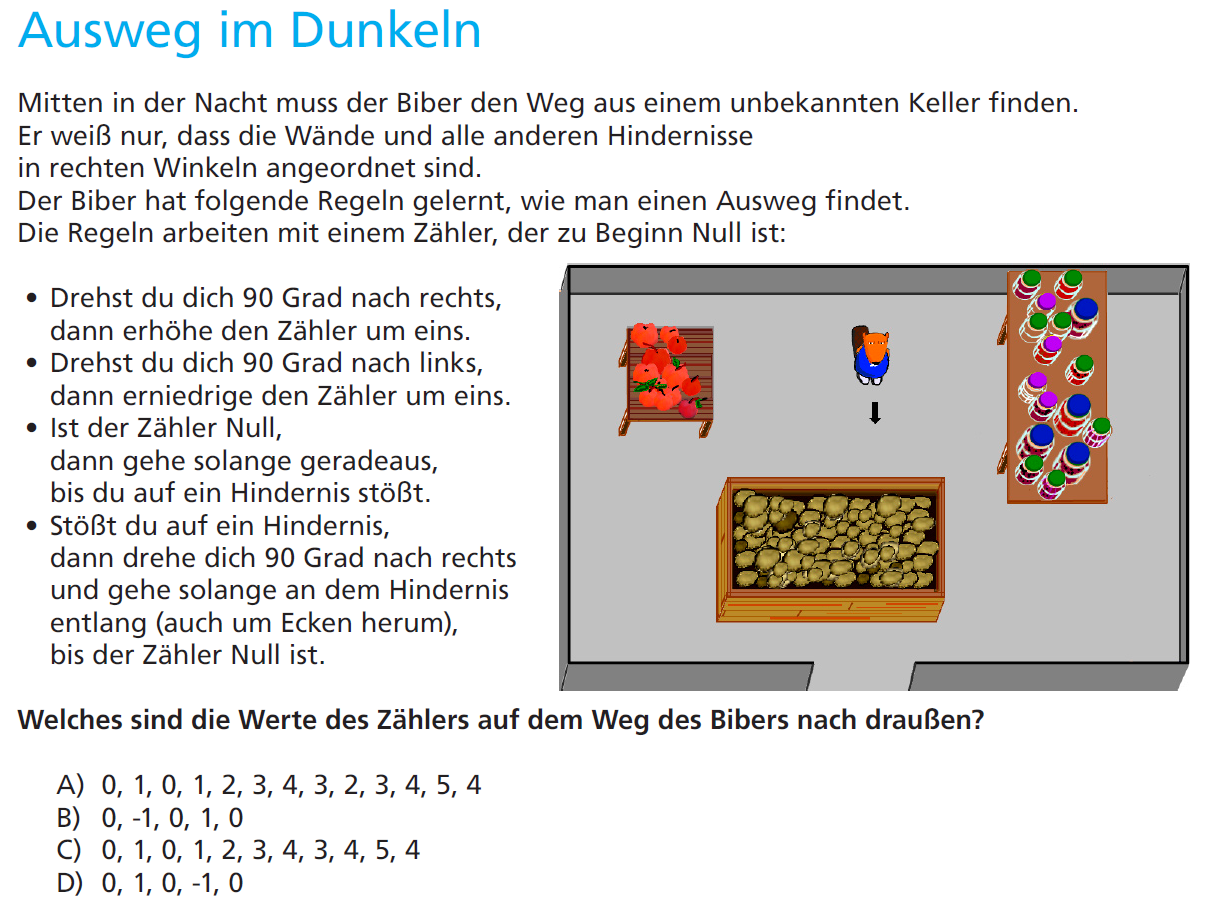
\includegraphics[height=8cm]{bild1.png}
\end{frame}

\begin{frame}[fragile]
Algorithmen zur Bestimmung des ggT (größter gemeinsamen Teiler)

Bestimmung des ggT von 28 und 52 durch Primfaktorzerlegung: \\
$28 =\pause 2 \cdot 2 \cdot 7$ \\
$52 =\pause 2 \cdot 2 \cdot 13$  \\
$\text{ggT}(28,52) = \pause4$

Bestimmung des ggT von 60 und 90 durch Primfaktorzerlegung: \\
$60 =\pause 2 \cdot 2 \cdot 3 \cdot 5$ \\
$90 =\pause 2 \cdot 3 \cdot 3 \cdot 5$ \\
$\text{ggT}(60,90) = \pause30$
\end{frame}

\begin{frame}[fragile]

\begin{lstlisting} 
# Algorithmus ggtDumm
Lies zwei positive ganze Zahlen ein
Setze ggt = erste Zahl
Solange nicht beide Zahlen durch ggt teilbar:
	erniedrige ggt um 1
Gib ggt aus
\end{lstlisting}    
Implementation in Python:  \pause

\begin{lstlisting} 
a = int(input())
b = int(input())
ggt = a
while (a % ggt != 0 or b % ggt != 0):
    ggt -=1
print(ggt)
\end{lstlisting} 

Implementation als Funktion:  \pause
\begin{lstlisting} 
def ggtDumm(a,b):
    ggt = a
    while (a % ggt != 0 or b % ggt != 0):
        ggt -=1
    return ggt
\end{lstlisting} 
\end{frame}

\begin{frame}[fragile]
\begin{minipage}[c]{8cm}
Beobachtung von Euklid: \\
Wenn $t$ Teiler von $a$ und $b$ ist, dann ist $t$ auch Teiler von $a-b$ (falls $a>b$).
\end{minipage} ~~
\begin{minipage}[c]{3cm}       \pause
\begin{tabular}{ll}
52  & 28 \\ \pause
24  & 28 \\ 
24  & 4 \\ 
20  & 4 \\ 
16 & 4 \\ 
12 & 4 \\ 
8 & 4 \\ 
4 & 4 \\ 
\end{tabular}
\end{minipage}

\begin{lstlisting} 
# Euklidscher Algorithmus
Ziehe von der größeren Zahl 
die kleinere ab, solange bis beide gleich sind.
\end{lstlisting}   \pause

\begin{lstlisting} 
def ggt(a,b):
    while a != b:
        if (a > b):
            a = a - b
        else:  
            b = b - a
    return a
\end{lstlisting}  
\end{frame}

\begin{frame}[fragile]
\begin{minipage}[c]{3cm}      
\begin{tabular}{ll}
128  & 34 \\
94 & 34 \\ 
60  & 34 \\ 
26 & 34 \\ 
26 & 8 \\ 
18 & 8 \\ 
10 & 8 \\ 
2 & 8 \\ 
2 & 6 \\
2 & 4 \\
2 & 2 \\
\end{tabular}
\end{minipage}
\begin{minipage}[c]{7cm}      
Beobachtung: Immer wenn die größere Zahl die Seiten wechselt, können wir die neue Zahl aus den beiden oberen berechnen. \pause

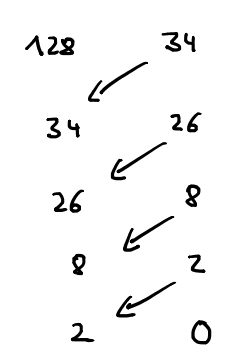
\includegraphics[scale=0.5]{bild2.png} \pause

\begin{lstlisting} 
# moderner euklidscher Algorithmus
def ggtTurbo(a,b):  
    while b != 0:
        a, b = b, a % b
    return a
\end{lstlisting} 
\end{minipage}

\end{frame}
 \end{document}
